\documentclass[a4paper, 11pt]{article}

%Math
\usepackage{amsmath}
\usepackage{amsfonts}
\usepackage{amssymb}
\usepackage{amsthm}
\usepackage{ulem}
\usepackage{stmaryrd} %f\UTF{00FC}r Blitz!

%PageStyle
\usepackage[ngerman]{babel} % deutsche Silbentrennung
\usepackage[ansinew]{inputenc} % wegen deutschen Umlauten
\usepackage{fontenc}
\usepackage{fancyhdr, graphicx} %for header/footer
\usepackage{wasysym}
\usepackage{fullpage}
\usepackage{textcomp}

% Listings
\usepackage{color}
\usepackage{xcolor}
\usepackage{listings}
\usepackage{caption}

\DeclareCaptionFont{white}{\color{white}}
\DeclareCaptionFormat{listing}{\colorbox{gray}{\parbox{\textwidth}{#1#2#3}}}
\captionsetup[lstlisting]{format=listing,labelfont=white,textfont=white}
 
\lstdefinestyle{JavaStyle}{
 language=Java,
 basicstyle=\footnotesize\ttfamily, % Standardschrift
 numbers=left,               % Ort der Zeilennummern
 numberstyle=\tiny,          % Stil der Zeilennummern
 %stepnumber=2,              % Abstand zwischen den Zeilennummern
 numbersep=5pt,              % Abstand der Nummern zum Text
 tabsize=2,                  % Groesse von Tabs
 extendedchars=true,         %
 breaklines=true,            % Zeilen werden Umgebrochen
 frame=b,         
 stringstyle=\color{white}\ttfamily, % Farbe der String
 showspaces=false,           % Leerzeichen anzeigen ?
 showtabs=false,             % Tabs anzeigen ?
 xleftmargin=17pt,
 framexleftmargin=17pt,
 framexrightmargin=5pt,
 framexbottommargin=4pt,
 showstringspaces=false      % Leerzeichen in Strings anzeigen ?        
}


%Metadata
\title{Algorithmen \& Datenstrukturen 2}
\author{Jan F�ssler}
\date{3. Semester (HS 2012)}
\fancyfoot[C]{If you use this documentation for a exam, you should offer a beer to the authors!}

% hier beginnt das Dokument
\begin{document}

% Titelbild
\maketitle
\thispagestyle{fancy}

\newpage

% Inhaltsverzeichnis
\pagenumbering{Roman}
\tableofcontents	  	


\newpage
\setcounter{page}{1}
\pagenumbering{arabic}

% Inhalt Start

\section{Listen}
Eine verkettete Liste (linked list) ist eine dynamische Datenstruktur zur Speicherung von Objekten. Sie eignen sich f�r das speichern einer unbakannten Anzahl von Objekten, sofern kein direkter Zugriff auf die einzelnen Objekte ben�tigt wird. Jedes Element in einer Liste muss neben den Nutzinformationen auch die notwendigen Referenzen zur Verkettung enthalten.\\ 
Es gibt drei verschiedene Arten von Listen:\\
\begin{center}
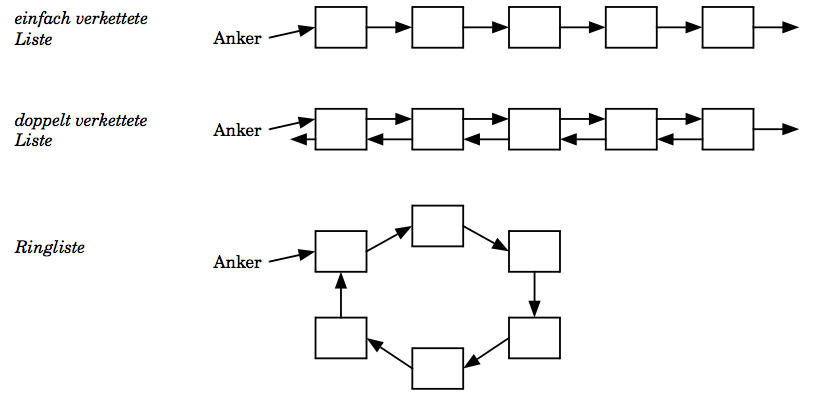
\includegraphics[scale=0.4]{listen.png}
\end{center}

\lstinputlisting[language=java,caption=Einfache verkettete Liste,style=JavaStyle]{linked_list.java}

\subsection{Stack}
Der Stack ist eine dynamische Datanstruktur bei der man nur auf das oberste Element des Stabels zugreifen (top), ein neues Element auf den Stabel legen (push) oder das oberste Element des Stapels entfernen (pop) kann.
\lstinputlisting[language=java,caption=Implementierung eines Stacks,style=JavaStyle]{stack.java}





% Inhalt Ende
\end{document}